\documentclass[12pt,letterpaper,boxed]{hmcpset}
\usepackage[margin=1in]{geometry}
\usepackage{enumerate}
\usepackage{graphicx}
\usepackage{amsmath}
\usepackage{mathtools}
\usepackage[mathscr]{euscript}
\usepackage{float}
\graphicspath{{images/}}

\name{Shaan Gareeb}
\class{State Estimation}
\assignment{9/29/2017}
%\duedate{9/29/2017}

\begin{document}
Code files chronological order (Not part of this paper but I wanted it to be documented somewhere)\\
stateEstimationTest3D\\
stateEstimationTest2D\\
stateEstimationTest2Dkf\\
stateEstimationTest3Dkf
\begin{center}
\textbf{Introduction}
\end{center}
This is a guide for those who have never done state estimation before. The idea behind state estimation is how to use sensor information to give the most accurate represenation of position and orientation. In this example we will start with a simple example of a 6DOF(degree of freedom) IMU which would give us accelerometer and gyroscope data. In the future I hope to expand to 9DOF which would include a magnetometer and then adding GPS.
\begin{center}
\textbf{Sensors}
\end{center}
\textbf{Accelerometer:} An accelerometer is a motion sensor which reports acceleration data in specific directions. They are small cantilever beams and are typically MEMS based. Typically a 3DOF accelerometer will report acceleration(units typically in a multiple of gravity, depends on the model) along the x y and z directions of the device (Directions usually specified on the IMU board). You can also purchase 1DOF accelerometers which will report acceleration in a single direction.\\\\
\textbf{Gyroscope:} A gyroscope is another motion sensor which reports angular velocity data(units usually rad/s but you will need to check the datasheet) about the x y and z directions of the device(Directions usually specified on the IMU board). Integrating the angular velocity data given by the gyroscope can give you the roll pitch and yaw of the device.\\\\
\textbf{IMU:} An IMU(Inertial Measurement Unit) is a device which packages various sensors onto one board. A 6DOF IMU typically incorporates a 3DOF accelerometer and a 3DOF gyroscope, while a 9DOF IMU will add on a 3DOF Magnetometer(Details to come)\\\\
\begin{center}
\textbf{State Estimation}
\end{center}
As discussed above state estimation is the process of using sensor data to give an accurate representation of position and orientation of a device. To understand the math in the portion below you should have a basic understanding of physics, matrices, and calculus.\\

We will first represent position on the cartesian coordinate frame. Position will be represented as $r$, where $r = [x\, y\, z]$ and $[x\, y\, z]$ are your positions along the 3 cartesian axes. Orientation will be represented as $\phi$ where $\phi = [\alpha\, \beta\, \gamma]$. $\alpha$ is the roll (rotation about the x axis) $\beta$ is the pitch (rotation about the y axis) $\gamma$ is the yaw (rotation about the z axis). With this orientation standard the forward direction is typically along the x axis.
\begin{figure}[H]
	\centering
	\textbf{Coordinate Axes}\par\medskip
	\fbox{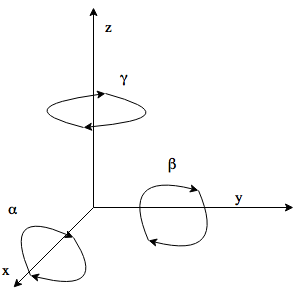
\includegraphics[scale=.7]{coordinateAxes}}
	\caption{Example of coordinate axes and orientation labeling}
\end{figure}

State estimation is all about converting data between the global and local coordinate frames. The global frame is typically the data we want to output, it is the position and orientation of our device with respect to a global origin point, if we were talking about a rocket this could be the launch pad with which the rocket launches from. The local frame is the data with respect to a local origin point which is typically the center of our IMU. 

\begin{figure}[H]
	\centering
	\textbf{Transformation}\par\medskip
	\fbox{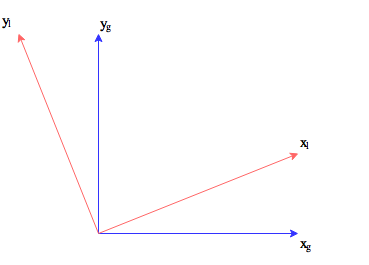
\includegraphics[scale=.7]{LocalToGlobalTransformation}}
	\caption{Transformation between local frame and global frame}
	\label{fig:transform}
\end{figure}
When we receive data from the IMU it is always in reference to the local frame. For example if I have an IMU on my rocket the x axis always points in the direction of the nose cone, no matter which way the rocket rotates in space or accelerates the x axis will always point along the nose cone. In this scenario the rockets x axis points vertically (because the rocket would be pointing up on the launchpad) , while the my x axis (or the global x axis) would be in some horizontal direction parallel to the ground. The question then becomes, how do I tell the rockets position in the global x axis? If I am standing at a launch pad, the rocket launches and moves 2 feet away from me in the global x direction, how am I going to know that if the IMU's local frame is so different from my global frame? The answer is in transformations. Using the rotational data from the gyroscope and the acceleration data from the accelerometer we can create rotational transformation matrices to rotate that data from its local frame to the global frame. 

\begin{center}
\textbf{Rotations}
\end{center}
Lets start with a simple rotation on a 2D axis. We will use x and y. Lets call the x and y magnitudes in the global frame $x_{g}$ and $y_{g}$, while the local frame magnitudes will be $x_{l}$ and $y{l}$. We will start with an example, lets say I have a point which is at (10,8) in the local frame, and I know the local frame has been rotated by 30 degree from the global frame. This example is shown in figure \ref{fig:example1}.

\begin{figure}[H]
	\centering
	\textbf{Transformation Example}\par\medskip
	\fbox{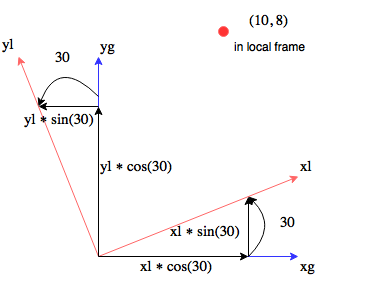
\includegraphics[scale=.7]{TransformationExample}}
	\caption{Example to transform a point from the local frame to the global frame}
	\label{fig:example1}
\end{figure}

Visually you can see that I would have to do some trigonometry to obtain my position in the global frame. First we want to see what my x coordinate would be in the global frame.

Because of the rotation the x component in the local frame exists on both sides of the y axis. So to figure out our global x component we will have to consider the part on the right side of the y axis as well as the left side of the y axis. We can first find the whole component as if it were to the right of the y axis by taking the magnitude of $x_{l}$ multiplied by $cos(\theta)$ which would be $10*cos(30)$. Now we need to subtract out the component to the left of the y axis. If you look carefully you can see that component is equivalent to the magnitude $y_{l}$ multipliled by $sin(\theta)$ which would be $8*sin(30)$.\\\\
We can use the same thought process to calculate the global y component. The global frame will be calculated in 2 parts, first we consider the contribution of the local y axis which is the magnitude of $y_{l}$ multiplied by $cos(\theta)$ or $8*cos(30)$. The second part is the contribution of the local x axis which is the magnitude of $x_{l}$ multiplied by $sin(\theta)$ or $10*sin(30)$. It might be difficult to understand from the explanation above, hopefully you can come to the same conclusion by looking at the figure. Finally you arrive at the equations below:\\

	\begin{align*}
	x_{g} &= 10*cos(30)-8*sin(30) \approx 4.66\\
	y_{g} &= 10*sin(30)+8*cos(30) \approx 11.93
	\end{align*}
From this we infer that the location of the point in the global frame is actually (4.66,11.93)
\begin{figure}[H]
	\centering
	\textbf{Global Frame Coordinate}\par\medskip
	\fbox{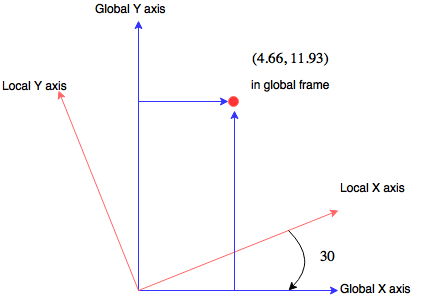
\includegraphics[scale=.7]{GlobalFrameCoordinate}}
	\caption{Final coordinate in the global frame}
	\label{fig:GlobalFrameCoordinate}
\end{figure}

Now that we have completed this example lets try generalizing the equations we came up with. Our rotation angle is $\theta$, local x and y magintudes are $x_{l}$ and $y_{l}$, and our global x and y magnitudes are $x_{g}$ and $y_{g}$.
	\begin{align*}
	x_{g} &= x_{l}cos(\theta)-y_{l}sin(\theta)\\
	y_{g} &= x_{l}sin(\theta)+y_{l}cos(\theta)
	\end{align*}
We can also put this into a matrix form:
\begin{math}
	\begin{bmatrix}
	x_{g}\\
	y_{g}
	\end{bmatrix}=
	\begin{bmatrix}
	cos(\theta)&-sin(\theta)\\
	sin(\theta)&cos(\theta)
	\end{bmatrix}*
	\begin{bmatrix}
	x_{l}\\
	y_{l}
	\end{bmatrix}
\end{math}\\
To generalize even further we can say: $r_{g} = R(\theta)*r_{l}$ where $r_{g}$ is my global position, $r_{l}$ is my local position, and $R(\theta)$ is called a rotation matrix. The conclusion here is that any point in the local frame can be converted to a point in the global frame via a rotational matrix, and all you need to keep track of is how the local frame has rotated ($\theta$) with respect to the global frame. In the next section we will cover 3 dimensional rotations.\\

\textbf{3D Rotations:} The 3D coordinate system has a third axis known as the z axis protruding out of the x-y plane. 3D rotations are the exact same thing as 2D rotations. If you think about it carefully the 2 dimensional rotation example that we did earlier was actually a 3D rotation about the z axis. When we do 3D rotations we are going to specify 2D rotations about each of the 3 axes then combine them into one matrix. You can try to derive them yourself using the technique we went through for the 2D rotations, but I will provide them in the list below:\\\\
\begin{math}
	R_x(\alpha) = 
	\begin{bmatrix}
	1&0&0\\
	0&cos(\alpha)&-sin(\alpha)\\
	0&sin(\alpha)&cos(\alpha)
	\end{bmatrix}\\\\
	R_y(\beta) = 
	\begin{bmatrix}
	cos(\beta)&0&sin(\beta)\\
	0&1&0\\
	-sin(\beta)&0&cos(\beta)
	\end{bmatrix}\\\\
	R_z(\gamma) = 
	\begin{bmatrix}
	cos(\gamma)&-sin(\gamma)&0\\
	sin(\gamma)&cos(\gamma)&0\\
	0&0&1
	\end{bmatrix}
\end{math}\\
Finally it can be shown that your total rotation matrix about all three axis is actually the multiplication of all 3 rotation matrices:
\begin{math}
R_{xyz}(\alpha,\beta,\gamma) = R_x(\alpha)*R_y(\beta)*R_z(\gamma)
\end{math}

\begin{center}
\textbf{Localization Algorithm}
\end{center}

This section will finally discuss how we use all of the techniques we learned thus far to convert IMU data into a position and orientation in the global frame. Back to the problem statement our IMU is fixed to the local frame but we care about the state of our device in the global frame. The first step is to provide our initial rotation matrix for the system, typically your device will start in a state of $\alpha = 0, \beta = 0, \gamma = 0$ thus we plug in those values and obtain our rotation matrix $R(\alpha,\beta,\gamma)$ and it would be equivalent to the identiy matrix.

The next step is to update our rotation matrix $R(t)$ given $\omega_L(t)$. There are two ways to accomplish this: 1) you can update your values for $\alpha, \beta, \gamma$ by integrating the rotational velocity measurements $\omega_L(t)$ then updating your rotation matrix with the new values. 2) Another slick way to update the rotation matrix is to generate a rotaional velocity matrix. The rotational velocity matrix $\Omega(t)$ can be shown to equal $\frac{dR(t)}{dt}$ or the derivative of the rotation matrix. To update the rotation matrix you just need to integrate this rotational velocity matrix which can be done using the following equation:
\begin{math}
	\Omega(t) =
	\begin{bmatrix}
	0&-\omega_z(t)&\omega_y(t)\\
	\omega_z(t)&0&-\omega_x(t)\\
	-\omega_y(t)&\omega_x(t)&0
	\end{bmatrix}\\\\
	R(t+\delta t) = R(t)[I+\Omega*\delta t]\\\\
$Then I normalized the rotation matrix by the cubic root of the determinant of the rotation matrix, that way the determinant of the resulting matrix would be one$\\\\
	R(t) = \frac{R(t)}{\sqrt[3]{det(R(t))}}\\\\
\end{math}
Now we can gather the orientation $(\alpha, \beta, \gamma)$ from our updated rotation matrix. You can go online to find formulas to back track the angles from the rotation matrix, or you could do the math yourself using the rotation matrix formulas shown above.\\
\begin{math}
\alpha = arctan(R_{3,2}(t),R_{3,3}(t))\\
\beta = arctan(R_{3,1}(t),\sqrt{R_{3,2}(t)^{2}+R_{3,3}(t)^{2}})\\
\gamma = arctan(R_{2,1}(t),R_{1,1}(t))
\end{math}

From here we use the update rotation matrix to convert the local acceleration to the global frame, then integrate to obtain position.\\
\begin{math}
a_g(t) = R(t)*a_l\\
$ (at this point if you were considering gravity you would subtract it from the z component of global acceleration)$\\
v_g(t) = v_g(t-1) +a_g(\delta t)\\
r_g(t) = r_g(t-1) + v_g(\delta t)
\end{math}

At this point we have generated position$(r_g(t))$ and orientation $(\alpha, \beta, \gamma)$ from the given local acceleration and local angular velocity data.\\

\begin{center}
\textbf{Example}
\end{center}
Lets consider an example set of data. I want my simulated drone to accelerate in the x direction for 1 second, at some point pitch then accelerate in the new direction for one second. The example data set will have $(a_{xl},a_{yl},a_{zl})$ for every time step as well as rotational velocity$(\omega_{x},\omega_{y},\omega_{x})$ about each axis in each time step.\\
\begin{math}
\begin{aligned}[c]
a_l &=(0,0,0)\\
&=(1,0,0) \\
&=(0,0,0) \\
&=(1,0,0) \\
&=(0,0,0) \\
&=(0,0,0) \\
&=(0,0,0) \\
&=(0,0,0) \\
&=(0,0,0) \\
&=(0,0,0) \\
&=(0,0,0) 
\end{aligned}
\begin{aligned}[c]
\omega &=(0,0,0) \\
&=(0,0,0) \\
&=(0,0,0) \\
&=(0,1.5,0) \\
&=(0,0,0) \\
&=(0,0,0) \\
&=(0,0,0) \\
&=(0,0,0) \\
&=(0,0,0) \\
&=(0,0,0) \\
&=(0,0,0) 
\end{aligned}
\end{math}

After running the code I get the following 3D plot:

\begin{figure}[H]
	\centering
	\textbf{Transformation}\par\medskip
	\fbox{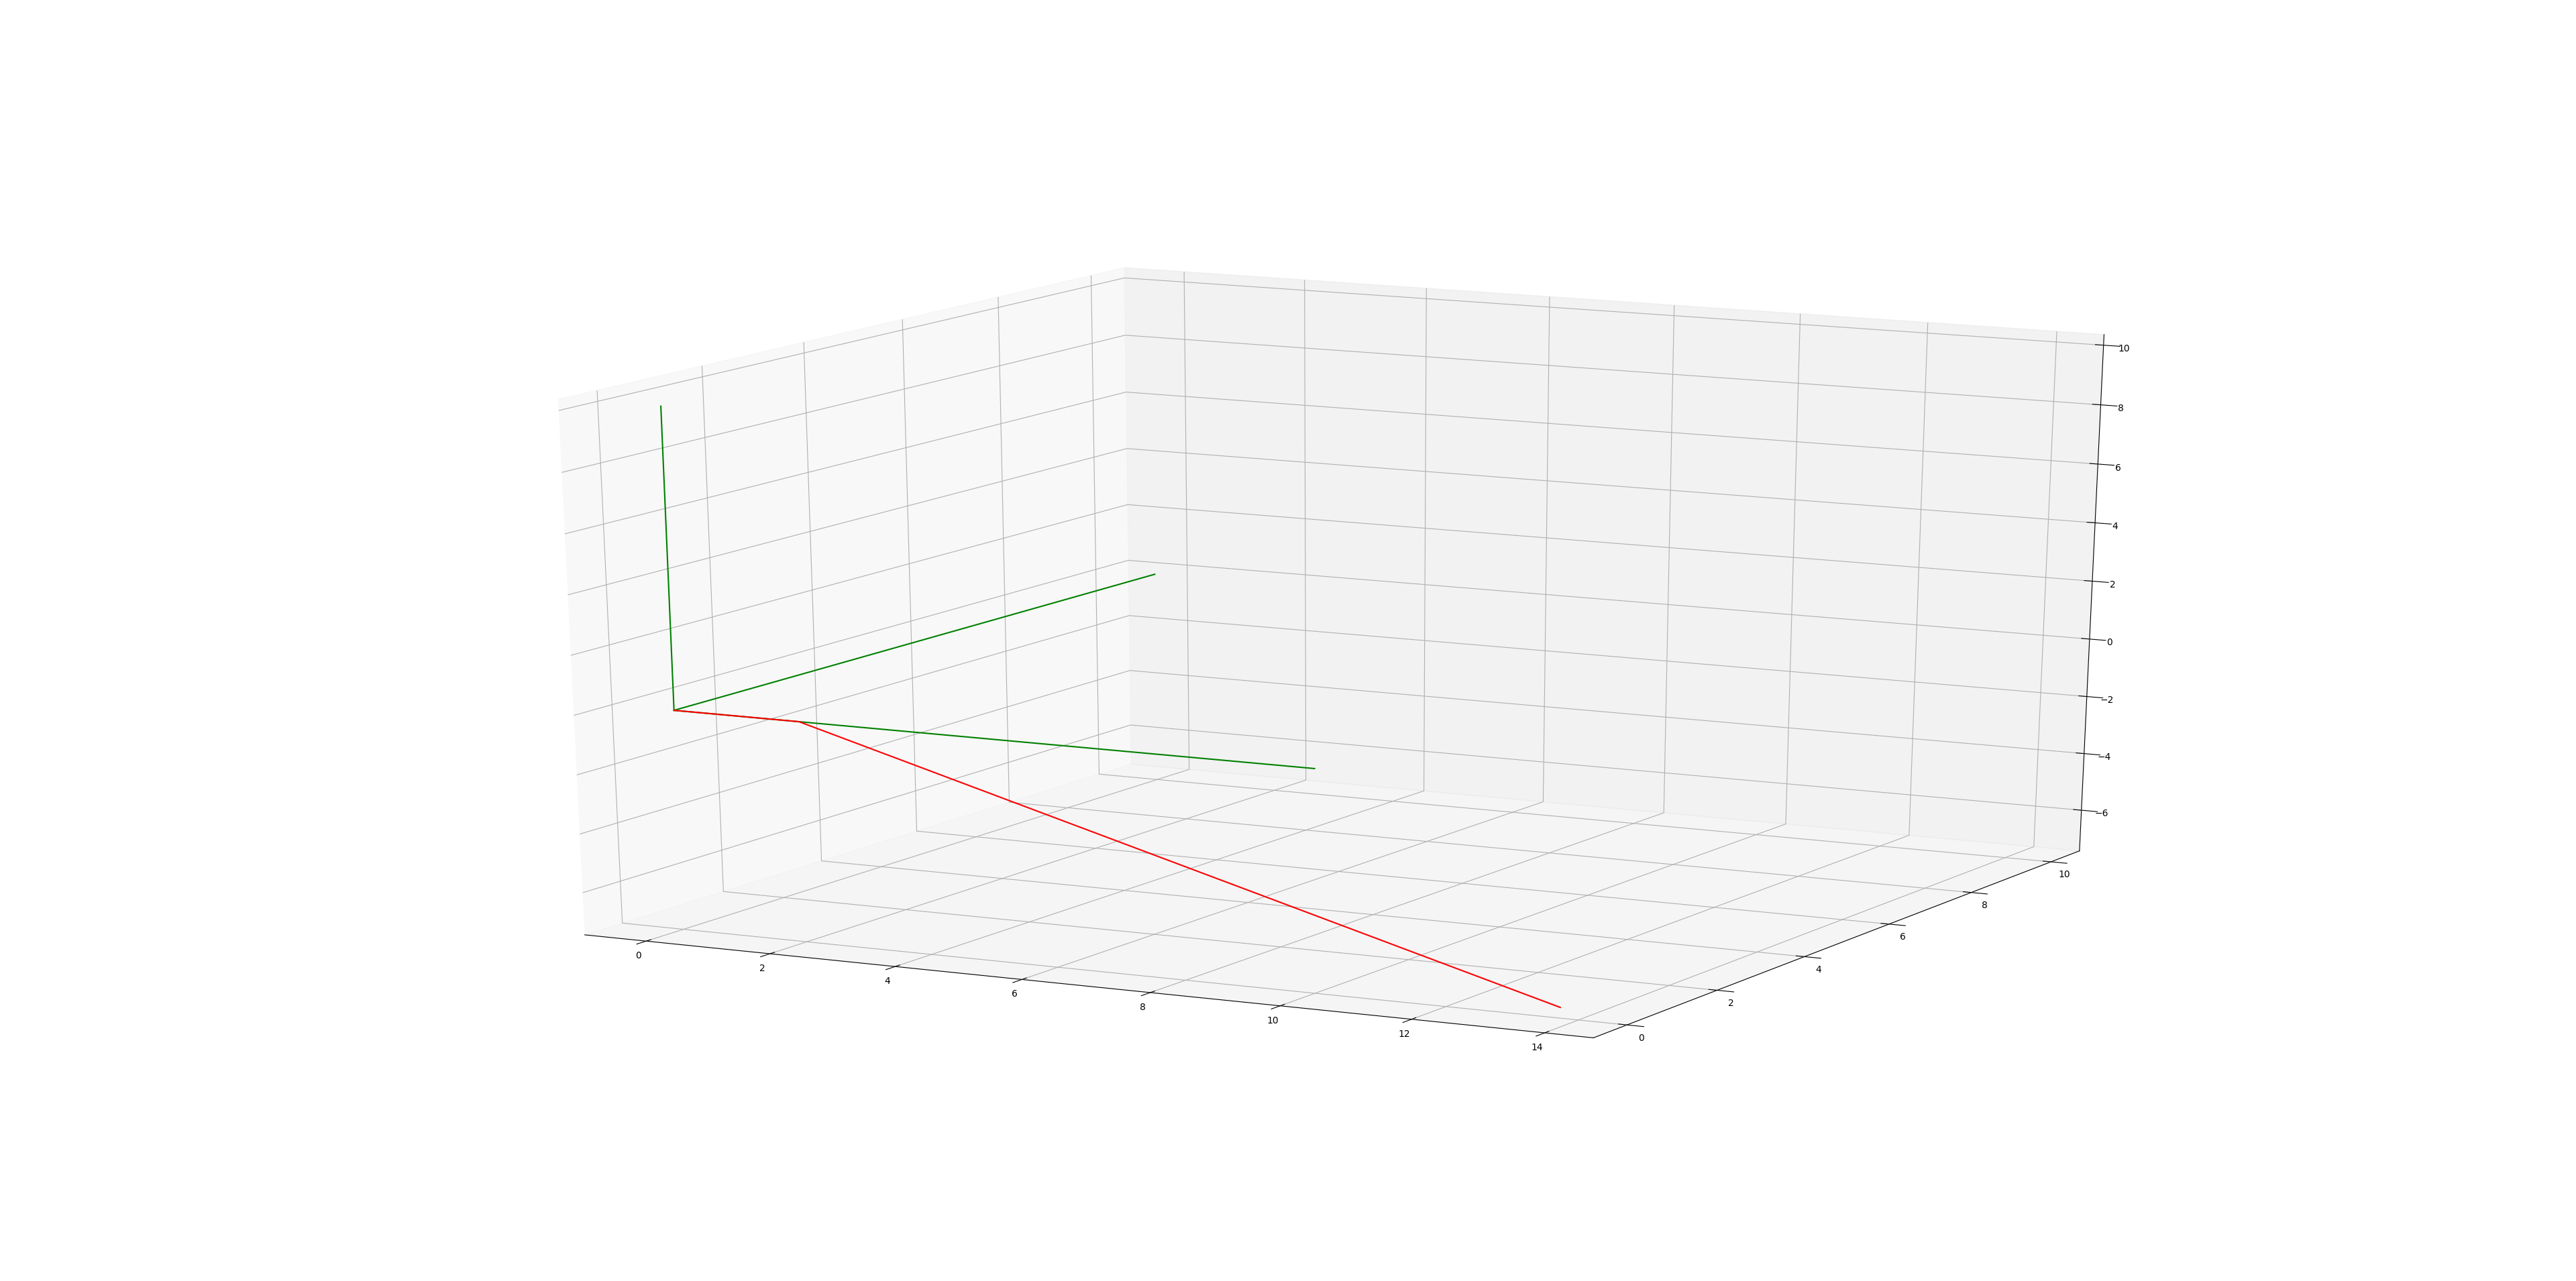
\includegraphics[scale=.15]{3DTestPlot}}
	\caption{3D plot of above data}
	\label{fig:3D}
\end{figure}

As you can see the the plot demonstrates the the drone went along an axis, pitched, then continued straight in the new direction.
%\newpage      Command to start a new page dont forget

\end{document}